\documentclass{standalone}
\usepackage{tikz}
\usetikzlibrary{patterns, positioning}
\usepackage[sfdefault]{ClearSans} %% option 'sfdefault' activates Clear Sans as the default text font
\usepackage[T1]{fontenc}

\begin{document}
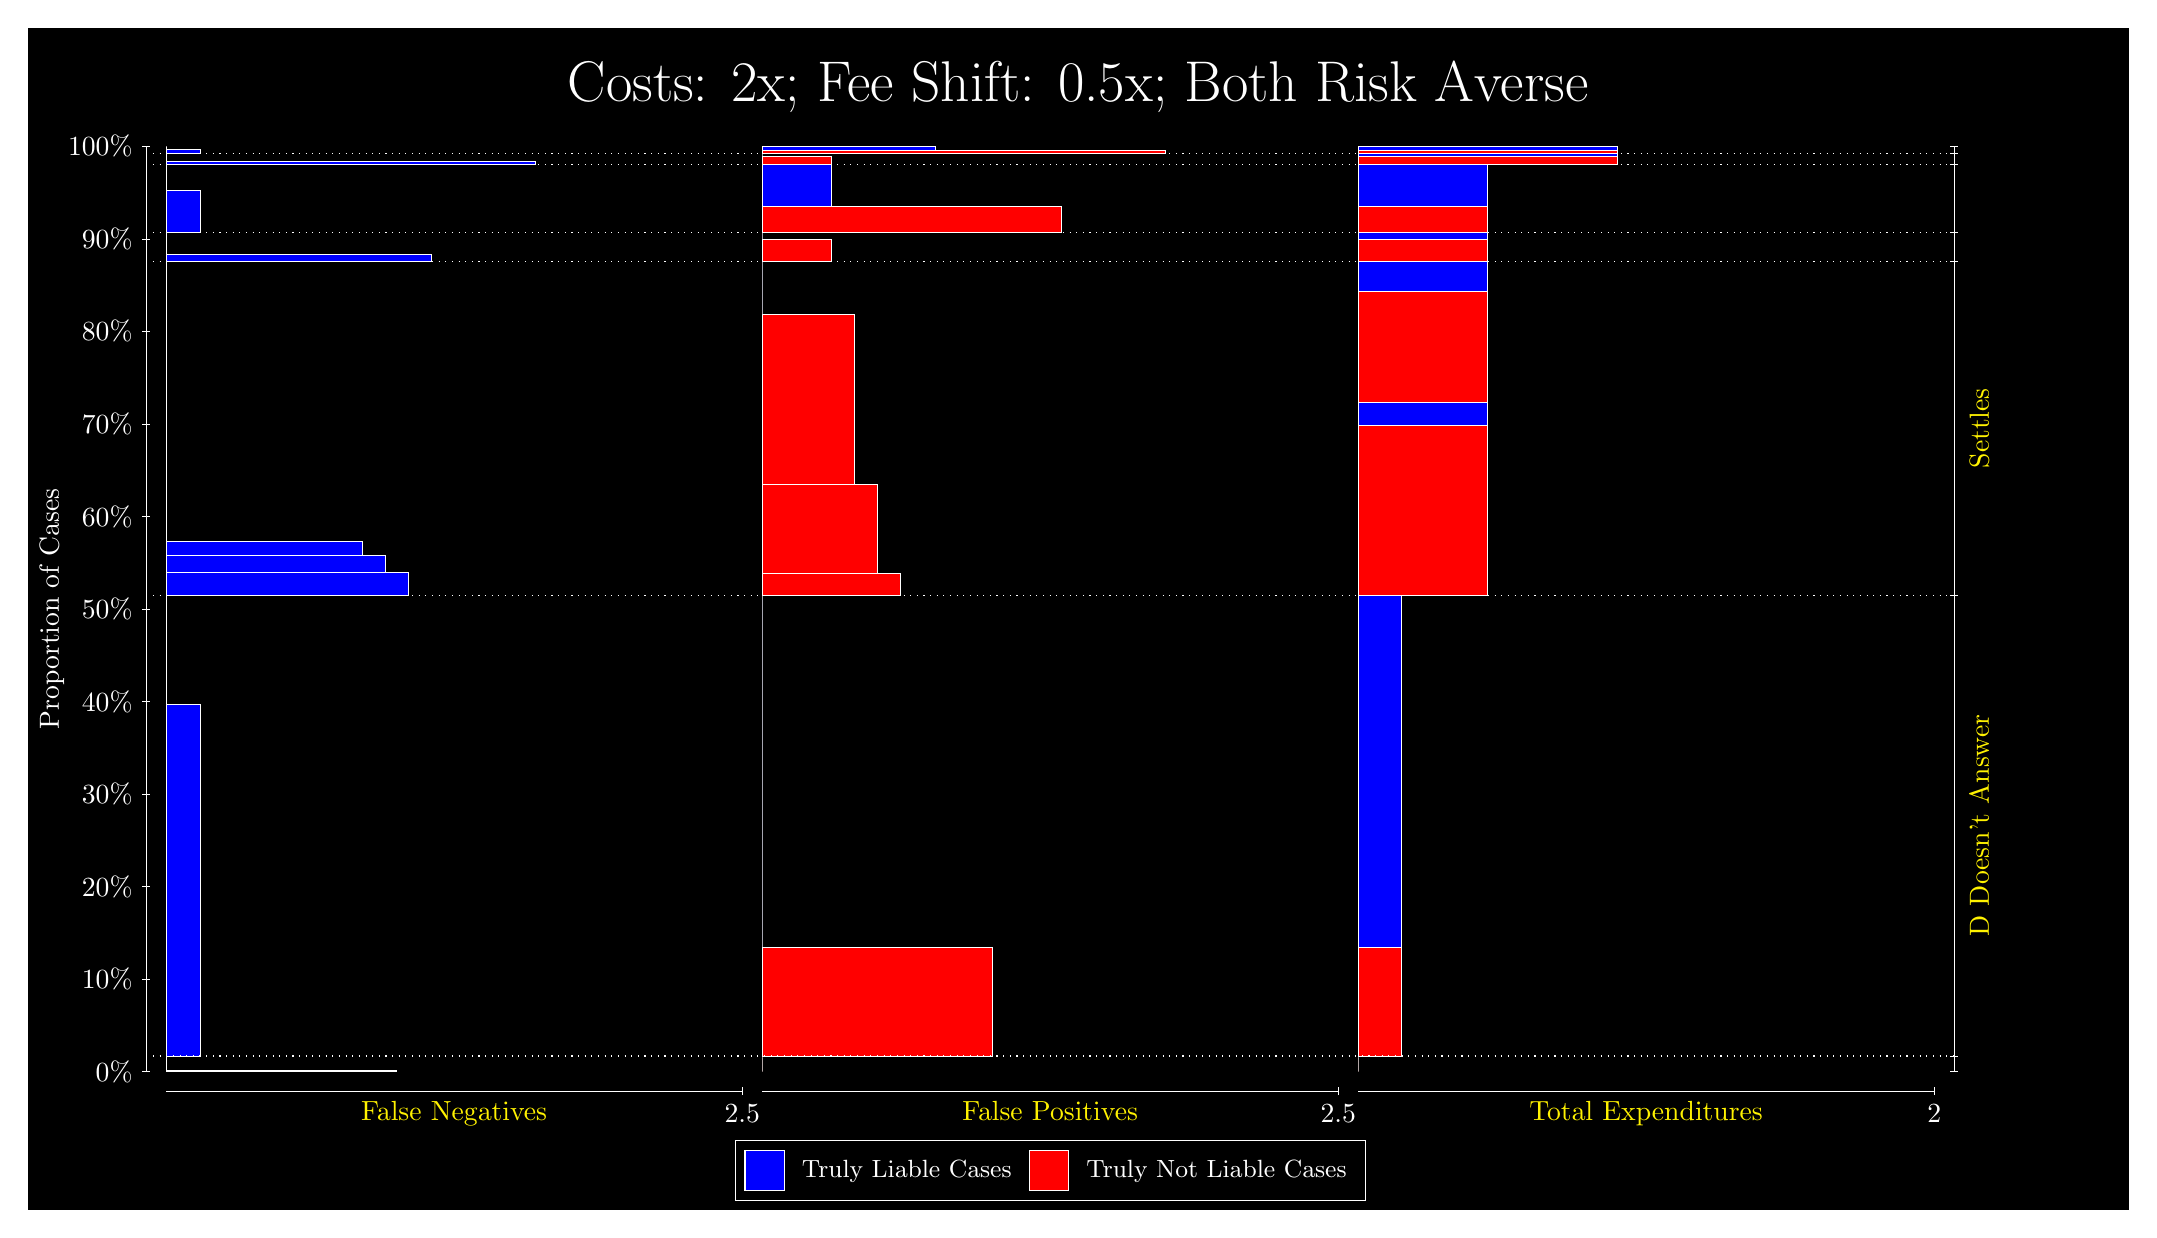
\begin{tikzpicture}
\draw[fill=black] (0,0) rectangle (26.667,15);
\draw[text=white] (0,13.5) rectangle (26.667,15) node[midway] {\huge Costs: 2x; Fee Shift: 0.5x; Both Risk Averse};
\draw[white, very thin] (1.5,1.75) -- (1.5,13.5);
\node[rotate=90, text=white, anchor=center] at (0.3, 7.625) {Proportion of Cases};
\draw[white, very thin] (1.45,1.75) -- (1.55,1.75);
\node[text=white, anchor=east] at (1.45, 1.75) {0\%};
\draw[white, very thin] (1.45,2.925) -- (1.55,2.925);
\node[text=white, anchor=east] at (1.45, 2.925) {10\%};
\draw[white, very thin] (1.45,4.1) -- (1.55,4.1);
\node[text=white, anchor=east] at (1.45, 4.1) {20\%};
\draw[white, very thin] (1.45,5.275) -- (1.55,5.275);
\node[text=white, anchor=east] at (1.45, 5.275) {30\%};
\draw[white, very thin] (1.45,6.45) -- (1.55,6.45);
\node[text=white, anchor=east] at (1.45, 6.45) {40\%};
\draw[white, very thin] (1.45,7.625) -- (1.55,7.625);
\node[text=white, anchor=east] at (1.45, 7.625) {50\%};
\draw[white, very thin] (1.45,8.8) -- (1.55,8.8);
\node[text=white, anchor=east] at (1.45, 8.8) {60\%};
\draw[white, very thin] (1.45,9.975) -- (1.55,9.975);
\node[text=white, anchor=east] at (1.45, 9.975) {70\%};
\draw[white, very thin] (1.45,11.15) -- (1.55,11.15);
\node[text=white, anchor=east] at (1.45, 11.15) {80\%};
\draw[white, very thin] (1.45,12.325) -- (1.55,12.325);
\node[text=white, anchor=east] at (1.45, 12.325) {90\%};
\draw[white, very thin] (1.45,13.5) -- (1.55,13.5);
\node[text=white, anchor=east] at (1.45, 13.5) {100\%};

\draw[white, very thin] (24.457,1.75) -- (24.457,13.5);
\draw[white, very thin] (24.407,1.75) -- (24.507,1.75);
\node[anchor=west] at (24.407, 1.75) {};
\draw[white, very thin] (24.407,1.9475) -- (24.507,1.9475);
\node[anchor=west] at (24.407, 1.9475) {};
\draw[white, very thin] (24.407,7.7993) -- (24.507,7.7993);
\node[anchor=west] at (24.407, 7.7993) {};
\draw[white, very thin] (24.407,12.042) -- (24.507,12.042);
\node[anchor=west] at (24.407, 12.042) {};
\draw[white, very thin] (24.407,12.406) -- (24.507,12.406);
\node[anchor=west] at (24.407, 12.406) {};
\draw[white, very thin] (24.407,13.272) -- (24.507,13.272);
\node[anchor=west] at (24.407, 13.272) {};
\draw[white, very thin] (24.407,13.414) -- (24.507,13.414);
\node[anchor=west] at (24.407, 13.414) {};
\draw[white, very thin] (24.407,13.5) -- (24.507,13.5);
\node[anchor=west] at (24.407, 13.5) {};

\draw[white, very thin, fill=blue] (1.75,1.75) rectangle (4.6775,1.7708);
\draw[white, very thin, fill=red] (1.75,1.7708) rectangle (1.75,1.9475);
\draw[white, very thin, fill=blue] (1.75,1.9475) rectangle (2.1891,6.4142);
\draw[white, very thin, fill=red] (1.75,6.4142) rectangle (1.75,7.7993);
\draw[white, very thin, fill=blue] (1.75,7.7993) rectangle (4.8239,8.0926);
\draw[white, very thin, fill=blue] (1.75,8.0926) rectangle (4.5312,8.3112);
\draw[white, very thin, fill=blue] (1.75,8.3112) rectangle (4.2384,8.48);
\draw[white, very thin, fill=red] (1.75,8.48) rectangle (1.75,12.042);
\draw[white, very thin, fill=blue] (1.75,12.042) rectangle (5.1167,12.129);
\draw[white, very thin, fill=red] (1.75,12.129) rectangle (1.75,12.406);
\draw[white, very thin, fill=blue] (1.75,12.406) rectangle (2.1891,12.939);
\draw[white, very thin, fill=red] (1.75,12.939) rectangle (1.75,13.272);
\draw[white, very thin, fill=blue] (1.75,13.272) rectangle (6.4341,13.309);
\draw[white, very thin, fill=red] (1.75,13.309) rectangle (1.75,13.414);
\draw[white, very thin, fill=blue] (1.75,13.414) rectangle (2.1891,13.464);
\draw[white, very thin, fill=red] (1.75,13.464) rectangle (1.75,13.5);
\draw[white, very thin, fill=red] (9.3189,1.75) rectangle (9.3189,1.9267);
\draw[white, very thin, fill=blue] (9.3189,1.9267) rectangle (9.3189,1.9475);
\draw[white, very thin, fill=red] (9.3189,1.9475) rectangle (12.246,3.3326);
\draw[white, very thin, fill=blue] (9.3189,3.3326) rectangle (9.3189,7.7993);
\draw[white, very thin, fill=red] (9.3189,7.7993) rectangle (11.075,8.0761);
\draw[white, very thin, fill=red] (9.3189,8.0761) rectangle (10.783,9.2082);
\draw[white, very thin, fill=red] (9.3189,9.2082) rectangle (10.49,11.361);
\draw[white, very thin, fill=blue] (9.3189,11.361) rectangle (9.3189,12.042);
\draw[white, very thin, fill=red] (9.3189,12.042) rectangle (10.197,12.319);
\draw[white, very thin, fill=blue] (9.3189,12.319) rectangle (9.3189,12.406);
\draw[white, very thin, fill=red] (9.3189,12.406) rectangle (13.125,12.739);
\draw[white, very thin, fill=blue] (9.3189,12.739) rectangle (10.197,13.272);
\draw[white, very thin, fill=red] (9.3189,13.272) rectangle (10.197,13.377);
\draw[white, very thin, fill=blue] (9.3189,13.377) rectangle (9.3189,13.414);
\draw[white, very thin, fill=red] (9.3189,13.414) rectangle (14.442,13.45);
\draw[white, very thin, fill=blue] (9.3189,13.45) rectangle (11.515,13.5);
\draw[white, very thin, fill=red] (16.888,1.75) rectangle (16.888,1.9267);
\draw[white, very thin, fill=blue] (16.888,1.9267) rectangle (16.888,1.9475);
\draw[white, very thin, fill=red] (16.888,1.9475) rectangle (17.437,3.3326);
\draw[white, very thin, fill=blue] (16.888,3.3326) rectangle (17.437,7.7993);
\draw[white, very thin, fill=red] (16.888,7.7993) rectangle (18.534,9.9524);
\draw[white, very thin, fill=blue] (16.888,9.9524) rectangle (18.534,10.246);
\draw[white, very thin, fill=red] (16.888,10.246) rectangle (18.534,11.655);
\draw[white, very thin, fill=blue] (16.888,11.655) rectangle (18.534,12.042);
\draw[white, very thin, fill=red] (16.888,12.042) rectangle (18.534,12.319);
\draw[white, very thin, fill=blue] (16.888,12.319) rectangle (18.534,12.406);
\draw[white, very thin, fill=red] (16.888,12.406) rectangle (18.534,12.739);
\draw[white, very thin, fill=blue] (16.888,12.739) rectangle (18.534,13.272);
\draw[white, very thin, fill=red] (16.888,13.272) rectangle (20.181,13.377);
\draw[white, very thin, fill=blue] (16.888,13.377) rectangle (20.181,13.414);
\draw[white, very thin, fill=red] (16.888,13.414) rectangle (20.181,13.45);
\draw[white, very thin, fill=blue] (16.888,13.45) rectangle (20.181,13.5);
\draw[white, dotted] (1.5,1.9475) -- (24.457,1.9475);
\draw[white, dotted] (1.5,7.7993) -- (24.457,7.7993);
\draw[white, dotted] (1.5,12.042) -- (24.457,12.042);
\draw[white, dotted] (1.5,12.406) -- (24.457,12.406);
\draw[white, dotted] (1.5,13.272) -- (24.457,13.272);
\draw[white, dotted] (1.5,13.414) -- (24.457,13.414);
\draw[white, very thin] (1.75,1.5) -- (9.0689,1.5);
\node[text=yellow, anchor=north] at (5.4094, 1.5) {False Negatives};
\draw[white, very thin] (9.0689,1.45) -- (9.0689,1.55);
\node[text=white, anchor=north] at (9.0689, 1.45) {2.5};

\draw[white, very thin] (9.3189,1.5) -- (16.638,1.5);
\node[text=yellow, anchor=north] at (12.978, 1.5) {False Positives};
\draw[white, very thin] (16.638,1.45) -- (16.638,1.55);
\node[text=white, anchor=north] at (16.638, 1.45) {2.5};

\draw[white, very thin] (16.888,1.5) -- (24.207,1.5);
\node[text=yellow, anchor=north] at (20.547, 1.5) {Total Expenditures};
\draw[white, very thin] (24.207,1.45) -- (24.207,1.55);
\node[text=white, anchor=north] at (24.207, 1.45) {2};


\node[text=yellow, centered, rotate=90] at (24.777, 4.8734) {D Doesn't Answer};
\node[text=yellow, centered, rotate=90] at (24.777, 9.9207) {Settles};





\draw (12.978300999999998,1.5) node[draw=none] (baseCoordinate) {};
\begin{scope}[align=center]
        \matrix[scale=0.5, draw=white, below=0.5cm of baseCoordinate, nodes={draw}, column sep=0.1cm]{
            \node[rectangle, draw, minimum width=0.5cm, minimum height=0.5cm, fill=blue] {}; &
            \node[draw=none, font=\small, text=white] (B) {Truly Liable Cases}; &
            \node[rectangle, draw, minimum width=0.5cm, minimum height=0.5cm, fill=red] {}; &
            \node[draw=none, font=\small, text=white] (B) {Truly Not Liable Cases}; \\
            };
\end{scope}

\end{tikzpicture}
\end{document}